% DRAFT of pre-readout-damage section for BB1GCR_note.tex.
% Insert before \section{Summary}. Error numbers below are FINAL (from damage_readout.npz).
% The one infidelity paragraph marked <<INFID>> is filled after recompute_damage_infid completes.

\section{Reading a pre-damaged codeword: when readout engineering stops helping}\label{sec:damage}

The noise analysis of Sec.~\ref{sec:mesolve} charged decoherence only to the readout
\emph{circuit}: the codeword entering each read is pristine, and the error is what the
finite-duration pulses accrue. A stored logical qubit faces the complementary hazard --- it
idles in the oscillator, accumulating photon loss and dephasing, \emph{before} the readout is
ever triggered. We now ask how each protocol reads a codeword that has \emph{already} been
damaged, isolating this input-damage axis from the readout-circuit noise studied above.

We prepare the canonical no-error logical-$0$ and logical-$1$ codewords --- the $\epsilon=0$
states of Sec.~\ref{sec:mesolve} --- and evolve each under a \emph{pure} oscillator
decoherence channel (zero Hamiltonian, a single collapse operator) for an idle time
$\tau\in[0,1000]\,\mu$s, before applying the readout with \emph{noiseless} pulses so that
every residual error is attributable to the input damage alone. Two channels are compared on a
common $\tau$-axis: oscillator photon loss $\sqrt{\kappa}\,\hat a$ at the Sivak-model rate
$\kappa=1/1000\,\mu\mathrm{s}^{-1}$ used throughout, and oscillator dephasing
$\sqrt{\kappa_\phi}\,\hat a^\dagger\hat a$ at $\kappa_\phi=1/5000\,\mu\mathrm{s}^{-1}$. The
Sivak model carries no intrinsic oscillator dephasing; we include it at a deliberately slower
rate as a qualitative comparison, not a calibrated hardware number. Figure~\ref{fig:damage}
tracks the readout error $P(e)$ and the post-read oscillator infidelity $1-F$ (after the same
single calibrated corrective displacement of Sec.~\ref{sec:mesolve}) against $\tau$, averaged
over the two codewords, which are symmetric under the channel.

The dominant message is a \emph{collapse of the protocol hierarchy}. At $\tau=0$ the seven
curves reproduce their noiseless operating points, spanning more than two orders of
magnitude --- from BB1(GCR) and the two blocks at $\sim\!10^{-5}$--$10^{-4}$, up through single
GCR ($6\times10^{-4}$), GCR-BB1 ($2.1\times10^{-3}$), to bare BB1 ($6.1\times10^{-3}$). Idle
photon loss erases this separation almost immediately: the spread is already inside a factor of
$\sim\!2$ by $\tau\approx170\,\mu$s (a sixth of the oscillator $T_1$), inside $10\%$ by
$\tau\approx500\,\mu$s, and by $\tau=1000\,\mu$s all seven agree to within $1\%$, clustered at
$P(e)\approx0.46$ --- just short of the $P(e)=\tfrac12$ random-guess limit. The reason is
physical: the logical bit is carried by the position-quadrature \emph{comb}, and photon loss
contracts and blurs that comb before any pulse acts. Once the lattice information has leaked out
of the input, no readout can recover it, and the choice of correction gadget becomes
irrelevant. Readout engineering buys accuracy only in the regime where the stored state is
still intact.

Dephasing is far gentler at these rates: it smears the comb in phase without contracting the
lattice, and at $\kappa_\phi=1/5000\,\mu\mathrm{s}^{-1}$ the error climbs only to
$P(e)\approx0.22$ by $\tau=1000\,\mu$s, with the hierarchy again collapsing --- the seven
protocols lie within $5\%$ of one another past $\tau\approx330\,\mu$s.

A subtler trend inverts the verdict of Sec.~\ref{sec:mesolve}. There, single GCR was the most
accurate readout because its short circuit accrued the least decoherence. Here, against a
\emph{pre-damaged} input, single GCR is instead the \emph{least} tolerant at intermediate
damage: at $\tau\approx170\,\mu$s it reads at $P(e)=0.087$ (photon loss) and $0.076$
(dephasing), while every BB1-structured scheme sits at $0.040$--$0.068$ and $0.061$--$0.074$
respectively. A single correction gives the narrowest correctable region, so a partially-decayed
input spills past it fastest; the multi-correction schemes, whose entire purpose is to widen
that region, absorb more of the damage-induced spread and degrade more gracefully. The effect
is modest and vanishes once the damage is severe, but it is the mirror image of the
readout-noise story: single GCR wins when the bottleneck is the readout \emph{circuit}, while
the correction-heavy schemes edge ahead when the bottleneck is a \emph{damaged input}.

% <<INFID>> paragraph -- fill from recompute_damage_infid output:
%   t=0 floor per scheme (should match fidelity table: GCR-BB1 1-F=0.023, blocks ~0.023-0.024,
%   BB1 ~higher); monotone rise toward 1 as state->vacuum; decay drives 1-F up faster than
%   dephasing; state whether ordering tracks P(e) or diverges.
The post-read oscillator infidelity tells the same story from the state's side.
%<<FILL>>

Together with Sec.~\ref{sec:mesolve}, this bounds the operational value of the whole
construction. The elaborate corrections earn their keep against readout-circuit noise, and buy
a modest graceful-degradation margin against a lightly-damaged input; but a heavily-damaged
codeword is a \emph{memory} failure, not a readout failure, and is beyond the reach of any
readout. The remedy there is a better oscillator or more frequent stabilization --- not a
longer pulse train.

\begin{figure}[tbp]
\centering
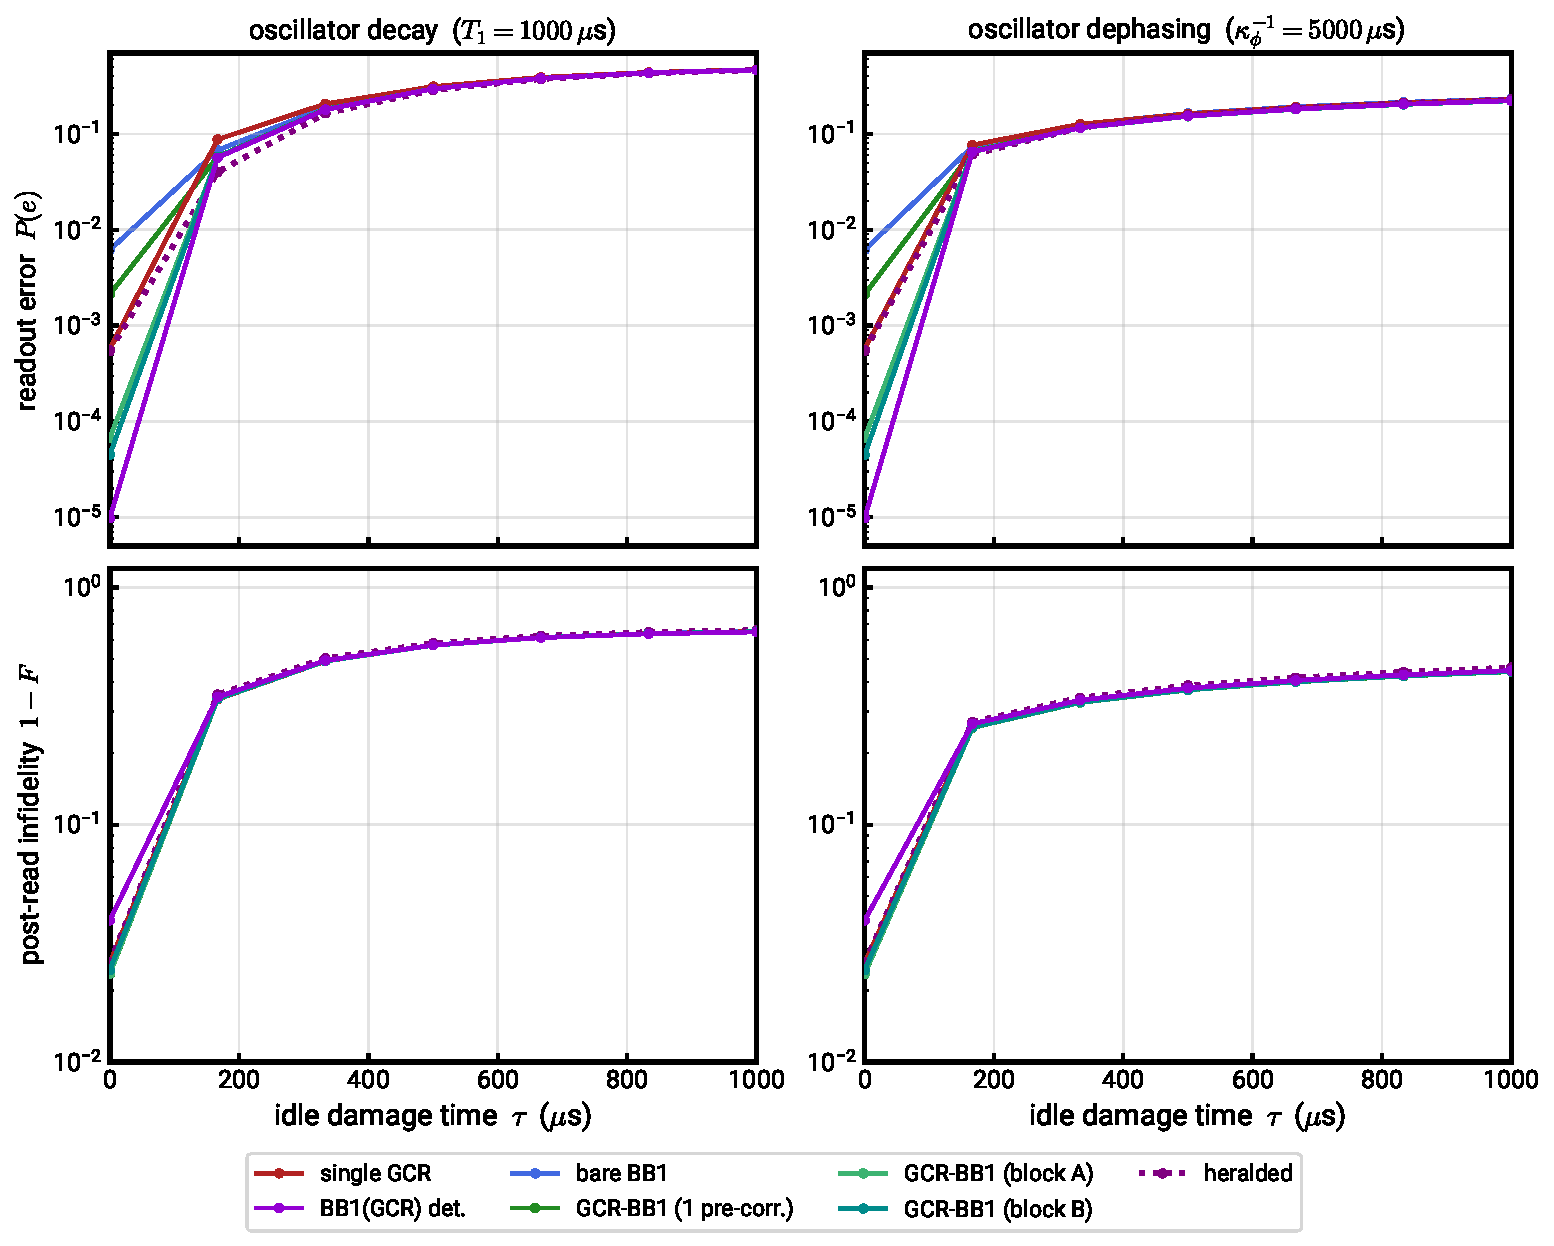
\includegraphics[width=0.92\textwidth]{Paper_Figures/damage_readout.pdf}
\caption{\textbf{Reading a pre-damaged codeword.} Undisplaced no-error logical-$0$/$1$ GKP
codewords are idled under a pure oscillator channel for time $\tau$ and then read with
\emph{noiseless} pulses, isolating the effect of input damage from readout-circuit noise.
Columns: oscillator photon loss ($T_1=1000\,\mu$s, left) and oscillator dephasing
($\kappa_\phi^{-1}=5000\,\mu$s, right). Top row: readout error $P(e)$; bottom row: post-read
oscillator infidelity $1-F$ after a single calibrated corrective displacement. Each panel
overlays the seven readout protocols (colors as in Figs.~\ref{fig:paired-readout} and
\ref{fig:paired-infidelity}); curves are averaged over the two codewords. The $\tau=0$ points
reproduce the noiseless operating points of Sec.~\ref{sec:mesolve}; under photon loss the
$>\!100\times$ spread among protocols collapses to within $1\%$ by $\tau=1000\,\mu$s, as the
lattice information leaks out of the input faster than any readout can extract it.}
\label{fig:damage}
\end{figure}
